\documentclass[varwidth]{standalone}

\begin{document}


\section{ZigZag Conversion (P006)}
\subsection{Pattern and Mapping}
First idea is find the pattern of the ZigZag conversion, as shown in
\cref{zigzag}.
\begin{figure}[H]
    \caption{ZigZag Example and Pattern}\label{zigzag}
    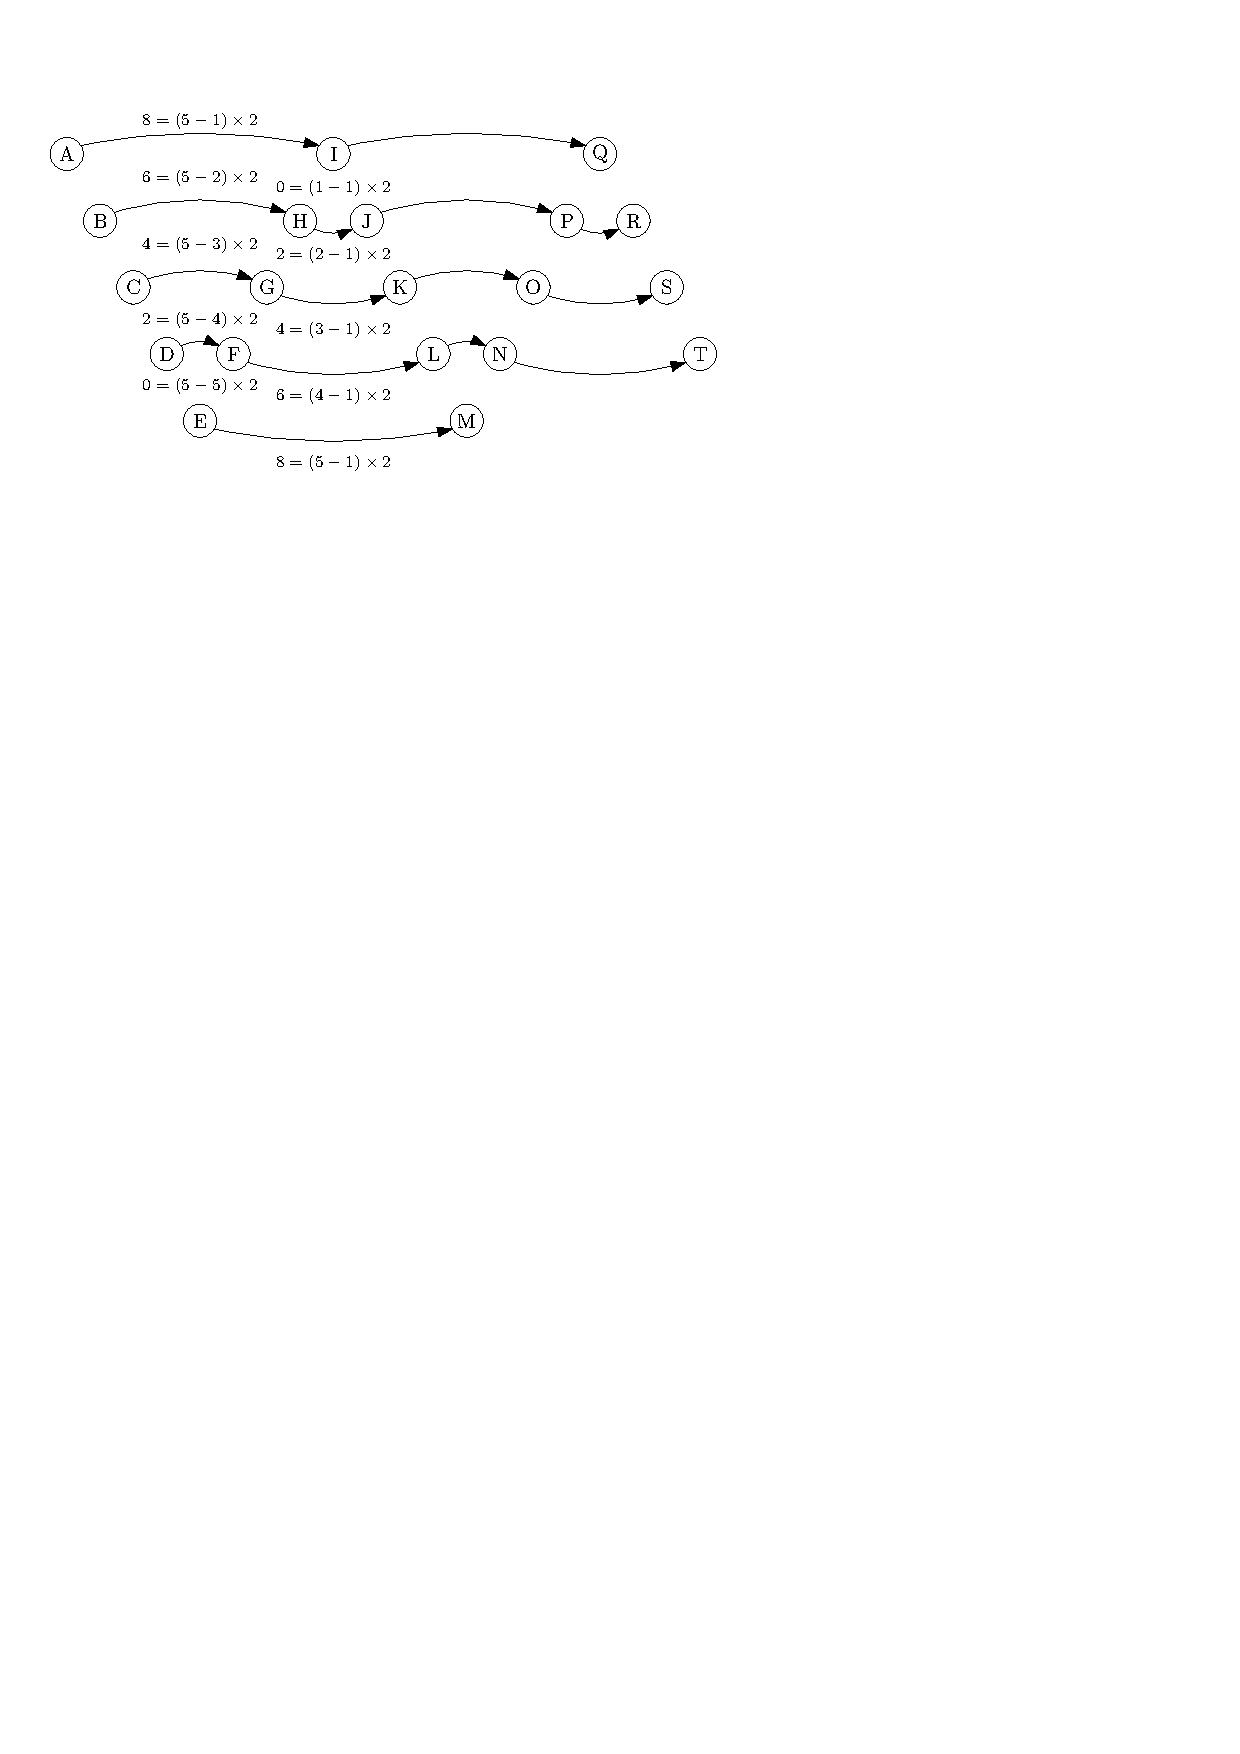
\includegraphics[width = \textwidth]{zigzag}
\end{figure}

It easy to see that for one round, there are $2 \times n - 1$ characters. At
each line, we need to take two step to get to the next round (consider the
first and last line take a `step' of zero step forward).
Furthermore, we can conclude the two step are as follow:
\begin{itemize}
    \item $Step1 = (NumOfRow - CurrentRow) \times 2$.
    \item $Step2 = (CurrentRow - 1) \times 2$.
\end{itemize}
Thus, we can directly traverse each line of the converted string,
find the corresponding characters from the original string and fill it in.

\subsection{Min Priority Queue}
View the problem in another aspect:
\begin{quote}
    When we traverse the original string, if we can determine the line number of
    each character in the ZigZag conversion, the line number can be used as a
    priority.

    By doing this, if we put all the character into a min priority queue,
    the sequence would naturally consistent with the ZigZag requirement, which
    characters with less line number would appear first.
\end{quote}

In addition, we need to ensure for characters with same line number, they are
FIFO in the min priority queue.
One way to achieve this is use the tuple of line number and index in original
string together as priority. For example (line, index) of (2, 4) should appear
before (2, 8).


My first implementation of this method is in python.
The solution turned out to be really slow.

Sad.

\end{document}

